\documentclass[11pt,a4paper,oneside]{report}
\usepackage[english,greek]{babel}
\usepackage[utf8x]{inputenc}
\usepackage[noend]{algpseudocode}
\usepackage{algorithm}
\usepackage{amssymb,latexsym,amsmath,ucs,amsthm,setspace,graphicx,fancyvrb,float}
\usepackage{hyperref}
\usepackage{tkz-graph}
\usepackage{subfig}
\newtheorem*{lemma}{Λήμμα}
\newcommand{\HRule}{\rule{\linewidth}{0.5mm}}
\newcommand{\defeq}{\overset{\underset{\mathrm{def}}{}}{=}}
\makeatletter
\DeclareMathOperator*{\argmin}{arg\,min}

\makeatother
\raggedbottom
\begin{document}

\begin{titlepage}
\begin{center}

\includegraphics[width=0.15\textwidth]{Pyrforos3.png}\\[1cm]
\textsc{\LARGE Εθνικό Μετσόβιο Πολυτεχνείο}\\[1.5cm]

\Large{ 3η Γραπτή Άσκηση }\\[0.5cm]

% Title
\begin{doublespace}
\HRule \\[0.4cm]
{\huge \bfseries
Αλγόριθμοι \& Πολυπλοκότητα
}\\[0.4cm]
\end{doublespace}

\HRule \\[1.5cm]

\begin{minipage}{0.4\textwidth}
\begin{flushleft} \large
\emph{Σπουδαστής:} \\
Διονύσης \textsc{Ζήνδρος} (06601)\\
\textlatin{\textless dionyziz@gmail.com\textgreater}
\end{flushleft}
\end{minipage}
\begin{minipage}{0.4\textwidth}
\begin{flushright} \large
\emph{Διδάσκοντες:} \\
Στάθης \textsc{Ζάχος}\\
Δημήτρης \textsc{Φωτάκης}
\end{flushright}
\end{minipage}

\vfill

{\large 24 Ιανουαρίου 2012}
\end{center}
\end{titlepage}

\section*{Άσκηση 1}
Το πρόβλημα μοντελοποιείται αν το αντιπροσωπεύσουμε με έναν γράφο στον οποίο κάθε ταινία είναι ένας κόμβος και κάθε συνδρομητής είναι μία ακμή ανάμεσα στις δύο ταινίες που θέλει να δει. Στη συνέχεια, αρκεί να χρωματίσουμε το γράφο με δύο χρώματα έτσι ώστε καμία ακμή να μην πατάει στο ίδιο χρώμα δύο φορές· με αυτό τον τρόπο ελέγχουμε αν ο γράφος μας είναι διμερής που είναι ουσιαστικά και το ζητούμενο του προβλήματος.

Για να ελέγξουμε αν ο γράφος είναι διμερής, χρωματίζουμε μία κορυφή αυθαίρετα και στη συνέχεια για κάθε χρωματισμένη κορυφή χρωματίζουμε τους γείτονές της με το αντίθετο χρώμα έως ότου ολοκληρωθεί η διαδικασία ή καταλήξουμε σε αντίφαση. 
Αυτό πρέπει να το επαναλάβουμε για κάθε συνεκτική συνιστώσα του γράφου μας.

\begin{lemma}
Ο αλγόριθμος ελέγχου διμερούς γράφου είναι ορθός.
\end{lemma}
\begin{proof}
Η ορθότητα του αλγορίθμου προκύπτει ως εξής. Ο αρχικός κόμβος κάθε συνιστώσας σε έναν έγκυρο διμερή διαχωρισμό, αν υπάρχει, μπορεί να χρωματιστεί αυθαίρετα. Στη συνέχεια, αν ο γράφος μας είναι πραγματικά διμερής, η αναζήτηση στη συγκεκριμένη συνιστώσα θα πρέπει να χρωματίσει με σωστό τρόπο όλους τους κόμβους χωρίς να αποτύχει. Άρα αν ο γράφος είναι πραγματικά διμερής, τότε ο χρωματισμός θα πρέπει να είναι επιτυχής. Αντίστροφα, αν έχουμε επιτυχή χρωματισμό, και επειδή κάθε χρώμα είναι αμετάκλητο, τότε θα έχουμε ελέγξει όλες τις ακμές για αντιφάσεις και καμία δεν θα έχει βρεθεί. Συνεπώς ο γράφος θα είναι διμερής. Αυτό ισχύει για κάθε συνεκτική συνιστώσα του γράφου και έτσι ολοκληρώνεται η απόδειξη.
\end{proof}

\selectlanguage{english}
\begin{algorithm}[H]
\caption{\textgreek{Άσκηση 1}}
\begin{algorithmic}[1]

\Procedure{Bipartite}{$V, E$}
    \State $unexplored \gets \{ V \}$
    \For {$v \in V$}
        \State $color[ v ] \gets \emptyset$
    \EndFor
    \While {$unexplored \neq \emptyset$}
    	\State $u \gets \text{an item of } unexplored$
        \State $unexplored \gets unexplored \setminus \{u\}$
        \State $S \gets \Call{EmptyStack}$
        \State $\Call{Push}{S, u}$
        \State $color[ u ] \gets \top$
        \While {$\lnot \Call{Empty}{S}$}
            \State $s \gets \Call{Pop}{S}$
            \State $unexplored \gets unexplored \setminus \{s\}$
            \State $paint \gets \lnot color[ s ]$
            \For {$\text{neighbour } t \text{ of } s$}
                \If {$color[ t ] \neq \emptyset$}
                    \If {$color[ t ] \neq paint$}
                        \State \Return $\bot$
                    \EndIf
                \Else
                    \State $color[ t ] \gets paint$
                    \State $\Call{Push}{S, t}$
                \EndIf
            \EndFor
        \EndWhile
    \EndWhile
    \State \Return $\top$
\EndProcedure
\end{algorithmic}
\end{algorithm}
\selectlanguage{greek}

Ο χρόνος εκτέλεσης του αλγορίθμου θα είναι $O( |V| + |E| )$. Αυτό προκύπτει από το γεγονός ότι διασχίζουμε όλες τις ακμές του γράφου από το πολύ δύο φορές, μία για κάθε άκρη τους, και άρα έχουμε $O( |E| )$, ενώ για κάθε συνιστώσα θα πρέπει να ξεκινήσουμε από κάποιον κόμβο της το οποίο κοστίζει $O( |V| )$.

\section*{Άσκηση 2}
Διασχίζουμε το γράφο χρησιμοποιώντας αναζήτηση κατά πλάτος και διατηρούμε κάθε φορά το πλήθος των τρόπων με τους οποίους φτάσαμε σε κάθε κόμβο.

\selectlanguage{english}
\begin{algorithm}[H]	
\caption{\textgreek{Άσκηση 2}}
\begin{algorithmic}[1]

\Procedure{ShortestCount}{$V, E, s, t$}
    \For {$v \in V$}
        \State $visited[ v ] \gets 0$
        \State $distance[ v ] \gets \infty$
    \EndFor
    \State $visited[ s ] \gets 1$
    \State $distance[ s ] \gets 0$
    \State $q \gets \Call{EmptyQueue}$
    \State $\Call{Enqueue}{q, s}$
    \While{$\lnot \Call{Empty}{q}$}
        \State $u \gets \Call{Dequeue}{q}$
        \If{$u = t$}
            \State \Return $visited[ t ]$
        \EndIf
        \For {$\text{neighbour } v \text{ of } u$}
            \If {$distance[ v ] = \infty$}
                \State $\Call{Enqueue}{q, u}$
            \EndIf
            \If {$distance[ u ] + 1 \leq distance[ v ]$}
                \State $distance[ v ] \gets distance[ u ] + 1$
                \State $visited[ v ] \gets visited[ v ] + visited[ u ]$
            \EndIf
        \EndFor
    \EndWhile
\EndProcedure
\end{algorithmic}
\end{algorithm}
\selectlanguage{greek}

Η πολυπλοκότητα του αλγορίθμου είναι η ίδια με αυτή της αναζήτησης κατά πλάτος, δηλαδή $O( |E| )$.

\section*{Άσκηση 3}
\subsection*{(α)}
Ο γράφος της άσκησης 4 με $L = \{ C \}$ είναι ένα παράδειγμα γράφου που έχει διαφορετικό ΕΣΔ υπό περιορισμούς.

\subsection*{(β)}
Για κάθε κόμβο για τον οποίο υπάρχει απαίτηση να είναι φύλλο κρατάμε την φθηνότερη ακμή που το συνδέει με κάποιον κόμβο που δεν υπάρχει απαίτηση να είναι φύλλο. Στη συνέχεια βρίσκουμε το ΕΣΔ κατά τα γνωστά.

\selectlanguage{english}
\begin{algorithm}[H]
\caption{\textgreek{Άσκηση 3}}
\begin{algorithmic}[1]

\Procedure{ConstraintedMST}{$V, E, L$}
	\If {$|V| \leq 2$}
	    \State \Return $E$
	\EndIf
    \For {$v \in V$}
        \State $adj[ v ] \gets \emptyset$
        \State $best[ v ] \gets \infty$
    \EndFor
    \For {$e = (u, v, w) \in E$}
    	\If {$u \not\in L \lor v \not\in L$}
            \If {$u \in L \lor v \in L$}
                \For {$s \in \{u, v\}$}
                    \If {$s \in L$}
                        \If {$w < best[ s ]$}
                            \State $best[ s ] \gets w$
                            \State $adj[ s ] \gets \{ e \}$
                        \EndIf
                    \EndIf
                \EndFor
            \Else
                \State $adj[ v ] \gets adj[ v ] \cup \{ e \}$
            \EndIf
        \EndIf
    \EndFor
    \State \Return $\Call{Prim}{V, adj}$
\EndProcedure
\end{algorithmic}
\end{algorithm}
\selectlanguage{greek}

Η πολυπλοκότητα του αλγορίθμου προκύπτει ως εξής. Για κάθε ακμή ενημερώνουμε την βέλτιστη ακμή που είναι γνωστή για κάποιο φύλλο, αν συνδέεται με κάποιο, σε σταθερό χρόνο. Ο συνολικός χρόνο γι' αυτό απαιτεί να περάσουμε από όλες τις ακμές σε συνολικό χρόνο $O( |E| )$. Ο αλγόριθμος του \textlatin{Prim} τρέχει σε $O(|E| + |V|\log|V|)$ που είναι και άνω φράγμα για όλο τον αλγόριθμο.

\section*{Άσκηση 4}
\subsection*{(α)}

Ο ακόλουθος γράφος έχει μοναδικό ΕΣΔ, αλλά περιέχει ακμές ίδιου βάρους:

\selectlanguage{english}
\begin{figure}[ht]
	\centering
		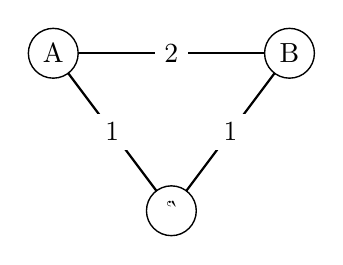
\begin{tikzpicture}
			\Vertex[x=0,y=0,L=A]{1}
			\Vertex[x=3,y=0,L=B]{2}
			\Vertex[x=1.5,y=-2,L=C]{3}

			\Edge[label=2](1)(2)
			\Edge[label=1](1)(3)
			\Edge[label=1](2)(3)
		\end{tikzpicture}
\end{figure}
\selectlanguage{greek}

\subsection*{(β)}
Ο γράφος του υποερωτήματος (α) έχει μοναδικό ΕΣΔ αλλά περιέχει ακμές ίδιου βάρους που είναι οι ελάχιστες που διασχίζουν το ίδιο κοψιμο.

\begin{lemma}
Κάθε ακμή ενός ΕΣΔ ενός συνεκτικού μη κατευθυνόμενου ζυγισμένου γράφου είναι η ελάχιστη που διασχίζει κάποιο κόψιμο.
\end{lemma}
\begin{proof}
Έστω τέτοιος γράφος $G = (V, E, w)$ με ένα ΕΣΔ του $T \subseteq E$ και έστω ότι υπάρχει κάποια ακμή $e = (u, v) \in T$ τέτοια ώστε να μην υπάρχει κόψιμο του G το οποίο να είναι η ελάχιστη που το διασχίζει. Τότε αφαιρώντας αυτή την τομή από το $T$ προκύπτει ένα κόψιμο $S$ του αρχικού γράφου σε δύο συνεκτικές συνιστώσες που είναι δέντρα. Το κόψιμο $S$ θα διασχίζεται από κάποια ακμή $f$ του $G$ που θα είναι ελάχιστη ακμή που διασχίζει το $S$. Επειδή η $e$ δεν είναι η ελάχιστη για κανένα κόψιμο, θα είναι $e \neq f$ και $w(f) < w(e)$. Όμως στο $T$ η ακμή $e$ μπορεί να αντικατασταθεί από την $f$ και το δέντρο να παραμείνει συνεκτικό και με βάρος $w( T \cup \{f\} \setminus \{e\}) < w( T )$. Άρα το $T$ δεν ήταν ΕΣΔ, κάτι το οποίο αποτελεί αντίφαση.
\end{proof}

\begin{lemma}
Κάθε συνεκτικός μη κατευθυνόμενος ζυγισμένος γράφος στον οποίο για κάθε κόψιμο η ακμή ελάχιστου βάρους που το διασχίζει είναι μοναδική έχει μοναδικό ΕΣΔ.
\end{lemma}
\begin{proof}
Έστω τέτοιος γράφος $G = (V, E, w)$ και δύο ΕΣΔ του, $T \subseteq E$ και $T' \subseteq E$,
με $T \neq T'$ και $w(T) = w(T')$.

Τότε, επειδή $T \neq T$, θα υπάρχει κάποια ακμή $e = (u, v)$ με $e \in T \land e \not\in T'$. Από το παραπάνω λήμμα, η $e$ θα είναι η ελάχιστη που διασχίζει κάποιο κόψιμο του $T$, έστω $S$.

Τώρα, επειδή το $T'$ είναι συνεκτικό δέντρο, θα υπάρχει μοναδικό μονοπάτι από τον κόμβο $u$ στον κόμβο $v$ που διασχίζει το $S$ με κάποια ακμή, έστω $e' \neq e$. Αφού $w(e) < w(e')$, αντικαθιστώντας την ακμή $e'$ με την $e$ στο $T'$ παίρνουμε ένα συνεκτικό δέντρο με βάρος $w(T' \cup\{e\} \setminus \{e'\}) < w(T')$. Άρα το $T'$ δεν είναι ελάχιστο συνεκτικό δέντρο, κάτι το οποίο αποτελεί αντίφαση.

Άρα το ΕΣΔ είναι μοναδικό.
\end{proof}

\subsection*{(γ)}
\begin{lemma}
Το ΕΣΔ ενός συνεκτικού ζυγισμένου μη κατευθυνόμενου γράφου είναι μοναδικό ανν κάθε ακμή του είναι η μοναδική ελάχιστη σε κάποιο κόψιμο του γράφου.
\end{lemma}

\begin{proof}
Έστω $G = (V, E, w)$ ένας τέτοιος γράφος και έστω $K$ ένα ΕΣΔ του.

Θα δείξουμε ότι αν κάθε ακμή του $K$ είναι η μοναδική ελάχιστη σε κάποιο κόψιμο, τότε το δέντρο είναι μοναδικό. Πράγματι, έστω ότι υπάρχει ΕΣΔ $T \neq K$. Τότε θα υπάρχει ακμή $e = (u, v) \in K \land e \not\in T$. Από την υπόθεση, υπάρχει κόψιμο $S$ το οποίο η $e$ διασχίζει ως μοναδική ελάχιστη. Επειδή το $T$ είναι συνδετικό, θα υπάρχει μοναδικό μονοπάτι που συνδέει τους κόμβους $u$ και $v$ το οποίο διασχίζει το κόψιμο $S$ χρησιμοποιώντας κάποια ακμή $f \neq e$. Επειδή η $e$ είναι ελάχιστη, θα είναι $w(e) < w(f)$. Αντικαθιστώντας την $f$ με την $e$ στο $T$ προκύπτει ΕΣΔ με $w( T \cup \{ e \} \setminus \{ f \} ) < w( T )$ κάτι το οποίο αποτελεί αντίφαση. Άρα το $K$ είναι μοναδικό.

Αντίστροφα, έστω ότι το $K$ είναι μοναδικό. Έστω, τώρα, ότι υπάρχει κάποια ακμή $e \in K$ που δεν είναι η μοναδική ελάχιστη σε κανένα κόψιμο του $G$. Τότε έστω το κόψιμο $S$ που δημιουργείται αν αφαιρέσουμε την $e$ από το $K$. Από το γεγονός ότι το $K$ είναι ελάχιστο (βλ. προηγούμενο θεώρημα), η $e$ θα είναι η ελάχιστη στο $S$. Έστω, τώρα, ότι υπάρχει και άλλη ελάχιστη ακμή $f \neq e$ που διασχίζει το $S$ με $w( f ) = w( e )$. Αντικαθιστώντας την $e$ με την $f$ στο $K$ παίρνουμε ένα συνδετικό δέντρο με βάρος $w( T \cup \{ f \} \setminus \{ e \} ) = w( T )$. Άρα το $K$ δεν ήταν μοναδικό συνδετικό δέντρο. Αυτό αποτελεί αντίφαση, και άρα όλες οι ακμές είναι ελάχιστες σε κάποιο κόψιμο.
\end{proof}

\subsection*{(δ)}
Ξεκινάμε υπολογίζοντας ένα ΕΣΔ του γράφου. Στη συνέχεια ελέγχουμε αν υπάρχει εναλλακτικό ΕΣΔ εργαζόμενοι ως εξής. Κατασκευάζουμε έναν πίνακα $V \times V$ που δείχνει τη μέγιστη ακμή του μονοπατιού ανάμεσα σε οποιουσδήποτε δύο κόμβους του ΕΣΔ. Τέλος, ελέγχουμε για κάθε ακμή του αρχικού γράφου $(u, v)$ αν μπορεί να αντικαταστήσει κάποια ακμή του ΕΣΔ και αυτό να παραμείνει ελάχιστο. Αυτό γίνεται πλέον εύκολα ελέγχοντας την τιμή της μέγιστης ακμής στο μονοπάτι από το $u$ στο $v$ πάνω στον αρχικό γράφο.

Η ορθότητα του αλγορίθμου προκύπτει άμεσα από το παρακάτω λήμμα:

\begin{lemma}
Ένα ΕΣΔ $T$ ενός συνδεδεμένου μη κατευθυνόμενου ζυγισμένου γράφου $G = (V, E, w)$ είναι μοναδικό ανν $\forall (u, v) \in E \setminus T: w( u, v ) > w(maxEdge(p(u, v)))$ όπου $p(u, v)$ το μονοπάτι από την κορυφή $u$ στην κορυφή $v$ στο δέντρο $T$.
\end{lemma}

\begin{proof}
Θα αποδείξουμε την ισοδυναμία με δύο αντίστροφες μεταξύ τους αποδείξεις με απαγωγή σε άτοπο.

Έστω ότι το $T$ δεν είναι μοναδικό, τότε θα υπάρχει $T' \neq T$ που διαφέρει κατά κάποια ακμή $e = (u, v)$ με $e \not\in T \land e \in T'$. Τότε έστω το κόψιμο $S$ που προκύπτει αν αφαιρέσουμε την $e$ από το $T'$. Αυτό το κόψιμο θα διασχίζει μια ακμή $f \neq e$ του $T$ που είναι μέρος του μοναδικού μονοπατιού που οδηγεί από την $u$ στη $v$ στο $T$ αφού το $T$ είναι ΕΣΔ. Οι $e$ και $f$ θα έχουν το ίδιο βάρος (βλ. παραπάνω θεώρημα) δηλαδή $w( e ) = w( f )$ διότι διαφορετικά τα $T$ και $T'$ δεν θα ήταν ελάχιστα. Άρα η $e$ δεν μπορεί να ξεπερνά το $w(maxEdge(p(u, v)))$. Αυτό είναι αντίφαση.

Αντίστροφα, έστω ότι υπάρχει ακμή $e = (u, v) \in E \setminus T$ τέτοια ώστε $w( e ) \leq w(maxEdge(p(u, v)))$ και έστω $f = maxEdge(p(u, v))$. Προφανώς θα είναι $e \neq f$. Τότε το $T \cup \{e\} \setminus \{f\}$ θα είναι συνδετικό δέντρο. Αν $w( e ) < w( f )$ τότε το νέο δέντρο έχει μικρότερο βάρος από το T, πράγμα αδύνατο. Άρα $w( e ) = w( f )$. Αντικαθιστώντας την $f$ με την $e$ στο $T$ προκύπτει ένα ΕΣΔ διαφορετικό από το αρχικό. Συνεπώς το $T$ δεν είναι μοναδικό. Αυτό είναι αντίφαση.

Τα δύο σκέλη αυτά μαζι ολοκληρώνουν την απόδειξη ισοδυναμίας.
\end{proof}

\selectlanguage{english}
\begin{algorithm}[H]
\caption{\textgreek{Άσκηση 4}}
\begin{algorithmic}[1]

\Procedure{UniqueMST}{$V, E, w$}
	\State $T \gets \Call{Prim}{V, E, w}$
	\For {$(u, v) \in V^2$}
		\State $dist[ u ][ v ] \gets \infty$
	\EndFor
	\For {$v \in V$}
		\State $q \gets \Call{EmptyStack}$
		\State $\Call{Push}{q,v}$
		\While {$\lnot \Call{Empty}{q}$}
			\State $u \gets \Call{Pop}{q}$
			\For {$\text{neighbour } r \text{ of } u \text{ in } T$}
				\If {$dist[ v ][ u ] = \infty$}
					\State $dist[ v ][ u ] \gets \max( dist[ v ][ r ], w( r, u ) )$
					\State $\Call{Push}{q,u}$
				\EndIf
			\EndFor
		\EndWhile
	\EndFor
	\For {$(u, v) \in E \setminus T$}
		\If {$w(u, v) = dist[ u ][ v ]$}
			\State \Return $\bot$
		\EndIf
	\EndFor
	\State \Return $\top$
\EndProcedure
\end{algorithmic}
\end{algorithm}
\selectlanguage{greek}

Ο αλγόριθμος του \textlatin{Prim} τρέχει σε $O( |V|^2 )$. Η κατασκευή του πίνακα μέγιστων ακμών ανά μονοπάτι μπορεί να γίνει σε χρόνο $O( |V|^2 )$ χρησιμοποιώντας αναζήτηση κατά πλάτος πάνω στο δέντρο. Η αναζήτηση ακμής αντικατάστασης γίνεται στη συνέχεια σε $O( |E| )$. Έτσι ο αλγόριθμος που προκύπτει είναι $O( |V|^2 )$.

\section*{Άσκηση 5}
\subsection*{(α)}
\begin{lemma}
Σε ένα συνεκτικό κατευθυνόμενο ζυγισμένο γράφο, για κάθε κύκλο υπάρχει ΕΣΔ που δεν περιέχει την ακμή μέγιστου βάρους του κύκλου αυτού.
\end{lemma}

\begin{proof}
Έστω τέτοιος γράφος $G = (V, E, w)$ με κάποιον κύκλο $C$ και έστω ένα ΕΣΔ $T \subseteq E$ που περιέχει την ακμή $e$ μέγιστου βάρους του $C$. Τότε έστω το δάσος $T \setminus \{ e \}$ που θα αποτελείται από δύο συνδεδεμένους υπογράφους. Θα υπάρχει μία ακμή $f \in E$ που θα συνδέει αυτούς τους δύο συνδεδεμένους υπογράφους με $f \neq e$ και άρα $w( f ) \leq w( e )$. Αντικαθιστώντας την $e$ με την $f$ στο $T$ προκύπτει ένα συνεκτικό δέντρο με βάρος $w( T \cup \{ f \} \setminus \{ e \} ) \leq w( T )$. Άρα το $T \cup \{ f \} \setminus \{ e \}$ είναι ΕΣΔ.
\end{proof}

\subsection*{(β)}
\begin{lemma}
Ο αντίστροφος αλγόριθμος του \textlatin{Kruskal} είναι ορθός.
\end{lemma}

\begin{proof}
Σε κάθε βήμα $i$, ο αλγόριθμος διατηρεί τον ελάχιστου κόστους συνδετικό υπογράφο $G_i$ με ακριβώς $j(i) = m - i + 1$ ακμές. Πράγματι, στο $1$ο βήμα, ο υπογράφος είναι ίσος με τον αρχικό γράφο και άρα συνδετικός και ελάχιστος. Έστω ότι ο υπογράφος είναι συνδετικός και ελάχιστος στο $i$-οστό βήμα. Τότε έστω $e = (u, v)$ η επόμενη ακμή που θα επιλεγεί.

Στην περίπτωση που η $e$ είναι γέφυρα του $G_i$ ανάμεσα σε δύο συνδεδεμένα τμήματα $C_1$ και $C_2$, δηλαδή διασχίζει το κόψιμο $S = ( C_1, C_2 )$ του αρχικού γράφου, η ακμή αυτή δε θα λείπει από κανέναν ελάχιστο συνδετικό υπογράφο $G_k$ με $k > i$. Αυτό φαίνεται ως εξής. Έστω ότι η $e$ έλειπε από τον $G_k$· τότε αυτός θα περιείχε κάποια ακμή $f \neq e$ που διασχίζει το $S$ για να είναι συνδεδεμένος. Όμως θα είναι $w(f) > w(e)$ διότι, λόγω άπληστης ιδιότητας, η $f$ είχε αφαιρεθεί πριν το $i$-οστό βήμα αφού η $e$ ήταν γέφυρα του $G_i$. Αντικαθιστώντας την $f$ με την $e$ λαμβάνουμε ένα συνδετικό υπογράφο ίδιου πλήθος ακμών με βάρος $w( G_k \cup \{ e \} \setminus \{ f \} ) < w( G_k )$. Άρα το $G_k$ δεν θα ήταν ελάχιστο χωρίς την ύπαρξη της $e$. Συνεπώς μπορούμε με ασφάλεια να διατηρήσουμε την $e$ στον υπογράφο και να προχωρήσουμε στην επόμενη ακμή στο ίδιο βήμα.

Στην περίπτωση που η $e$ δεν είναι γέφυρα του $G_i$, τότε ανήκει σε ένα κύκλο του $G_i$. Εργαζόμενοι παρόμοια όπως στο παραπάνω θεώρημα, είναι εμφανές ότι η $e$ δεν ανήκει στον υπογράφο $G_{i+1}$. Την αφαιρούμε, λοιπόν, και προχωράμε στο επόμενο βήμα.

Χρησιμοποιώντας, τώρα, τη μαθηματική επαγωγή, έχουμε αποδείξει την αμετάβλητη ιδιότητα της επανάληψης. Τέλος, ο ελάχιστος συνδετικός υπογράφος με ακριβώς $n - 1$ ακμές είναι ΕΣΔ.
\end{proof}

\subsection*{(γ)}

\selectlanguage{english}
\begin{algorithm}[H]
\caption{\textgreek{Άσκηση 5}}
\begin{algorithmic}[1]

\Procedure{ReverseKruskal}{$V, E, w$}
	\State $E \gets \text{sort } E \text{ decreasingly by weight}$
	\State $S \gets E$
	\For {$e \in E$}
		\If {$\lnot \Call{Bridge}{S, e}$}
			\State $S \gets S \setminus \{ e \}$
		\EndIf
	\EndFor
	\State \Return $S$
\EndProcedure
\end{algorithmic}
\end{algorithm}
\selectlanguage{greek}

Η υλοποίηση του \selectlanguage{english}$\Call{Bridge}{S, e}$\selectlanguage{greek} ελέγχει αν η $e$ είναι γέφυρα του $S$ και μπορεί να γίνει με διάφορους τρόπους. Ο απλούστερος τρόπος θα ήταν ένας αλγόριθμος αναζήτησης κατά βάθος ή κατά πλάτος που ελέγχει αν υπάρχει και άλλο μονοπάτι ανάμεσα στις δύο κορυφές που συνδέει η ακμή. Τότε η συνολική πολυπλοκότητα του αλγορίθμου είναι $O( E^2 )$. Αντικαθιστώντας τον έλεγχο για γέφυρες με κάποια πιο αποδοτική υλοποίηση (βλ. \cite{thorup00}) μπορούμε να πετύχουμε την αισθητά καλύτερη πολυπλοκότητα $ O(E \log E (\log \log E)^3) $.

\begin{thebibliography}{9}

\selectlanguage{english}

\bibitem{thorup00}
  Mikkel Thorup,
  \emph{Near-optimal fully-dynamic graph connectivity}.
  Addison Wesley, Massachusetts,
  Proc. 32nd ACM Symposium on Theory of Computing,
  2000.
  
\end{thebibliography}

\end{document}
